%
% Another appendix chapter
\chapter{Constrained Orbital Energy Trajectories}\label{chap:mpc}
The height constrained capture bounds cannot be used directly in control, as they consider impacts with no constraints on force. The force constrained bang-bang control law has to be integrated numerically to have knowledge of future states. Therefore, it is interesting to explore an additional method that has knowledge over future states, without the drawback of numerical integration. This chapter proposes an extension to the work of Koolen, Posa and Tedrake in \cite{koolen2016balance}, which relies for an important part on the work by Pratt and Drakunov in \cite{pratt2007derivation}: the \textit{orbital energy} of the \ac{VHIP}.

%% Constraint matrix/polynomial
\section{Constraint Matrix with Final Velocity}
In \cite{koolen2016balance}, the final horizontal velocity $\dot{x}_f$ is set to zero, as this leads to a \textit{capture trajectory}: a trajectory that leads to convergence to the unstable equilibrium of the \ac{VHIP}. However, the trajectories are unconstrained and can become unrealistically high above the ground, as shown in \figref{fig:cpbal}. To take kinematic limits of the system into account, constraints on the configuration of the \ac{VHIP} have to be added. In this section, the final horizontal velocity of the \ac{VHIP} orbital energy is left undetermined, and used to find trajectories that do not violate kinematic constraints.

Leaving the final horizontal velocity open can be used in constrained optimization. Using the \ac{VHIP} orbital energy of Equation \ref{eq:evhip}, but setting the final horizontal position zero gives:
\begin{equation}
    \frac{1}{2}\dot{x}^2\bar{f}^2(x)+gx^2f(x) - 3g\int_{0}^xf(\xi)\xi d\xi = \frac{1}{2}\dot{x}_0^2\bar{f}^2(0).
\end{equation}
Note that $\bar{f}^2(0)=(f(0)-f'(0) \cdot 0)^2=f(0)^2$. The additional nonzero term on the right-hand side can be added in the constraint matrix of \cite{koolen2016balance}. The constraint matrix reads as:
\begin{equation}
    \underbrace{\begin{bmatrix}1 & 0 & 0 & 0 \\ 
     1 & x_0 & x_0^2 & x_0^3\\
     0 & 1 & 2x_0 & 3x_0^2\\
     \frac{3}{2}gx_0^2 & gx_0^3 & \frac{3}{4}gx_0^4 & \frac{3}{5}gx_0^5\\
     \end{bmatrix}}_{\matr{A}}
     \underbrace{\begin{bmatrix}
     c_0\\
     c_1\\
     c_2\\
     c_3\\
     \end{bmatrix}}_{\vect{c}}=
     \underbrace{\begin{bmatrix}
     z_f\\
     z_0\\
     \frac{\dot{z}_0}{\dot{x}_0}\\
     k\\
     \end{bmatrix}}_{\vect{b}},
     \label{eq:amatrix}
\end{equation}
where $\matr{A}$ is the constraint matrix, $\vect{c}$ is the vector containing the polynomial constants and $\vect{b}$ is the constraint vector, giving a constraint on final height, initial height, initial direction and conservation of orbital energy respectively.
%$f(x)=\sum_{i=0}^3 c_ix^i$. 
The parameter $k$ in $\vect{b}$ is derived as follows. The integral term in the orbital energy equation, written as a cubic polynomial, read as: $3g\int_{0}^xf(\xi)\xi d\xi = 3g\sum_{i=0}^3\frac{1}{i+2}c_ix_0^{i+2}$. The last constraint of Equation \ref{eq:amatrix} reads after addition of the final velocity term as:
\begin{equation}
		3g\int_{0}^xf(\xi)\xi d\xi =\frac{1}{2}\dot{x}^2\bar{f}^2(x)+gx^2f(x) - \frac{1}{2}\dot{x}_0^2\bar{f}^2(0),
\end{equation}
and in terms of the cubic polynomial as:
\begin{align}
	3g\sum_{i=0}^3\frac{1}{i+2}c_ix_0^{i+2}& = \frac{1}{2}(\dot{x}_0z_0-\dot{x}_0x_0)^2 + gx_0^2z_0 - \frac{1}{2}z_f^2\dot{x}_f^2,\\
	&=k,
\end{align}
where $k$ is the last entry of vector $\vect{b}$. 

Using the polynomial description, and having a nonzero final velocity $\dot{x}_f$, the final height constraint $z_f$ results in a final height velocity $\dot{z}_f$ relative to the gradient of the polynomial at $x_f=0$:
\begin{align}
 	f'(0) &= \frac{\dot{z}_f}{\dot{x}_f},\\
 	\dot{z}_f &= f'(0)\dot{x}_f.
\end{align}
It could be undesirable that $\dot{z}_f$ is depending on $\dot{x}_f$. When $\dot{x}_f \neq 0$, additional future actions have to be taken, like taking a step, to come to a stop. High vertical velocities can result in for example high impacts, which can be undesirable. Therefore, it could be useful to have zero height velocity at this point. The constraint $f(0)=z_f$ in the first row in Equation \ref{eq:amatrix} can be replaced with the following constraint:
\begin{equation}
    \underbrace{\begin{bmatrix}0 & 1 & 0 & 0 \\ 
     1 & x_0 & x_0^2 & x_0^3\\
     0 & 1 & 2x_0 & 3x_0^2\\
     \frac{3}{2}gx_0^2 & gx_0^3 & \frac{3}{4}gx_0^4 & \frac{3}{5}gx_0^5\\
     \end{bmatrix}}_{\matr{A}}
     \underbrace{\begin{bmatrix}
     c_0\\
     c_1\\
     c_2\\
     c_3\\
     \end{bmatrix}}_{\vect{c}}=
     \underbrace{\begin{bmatrix}
    \frac{\dot{z}_f}{\dot{x}_f}\\ 
     z_0\\
     \frac{\dot{z}_0}{\dot{x}_0}\\
     k\\
     \end{bmatrix}}_{\vect{b}}
     \label{eq:a1matrix}
\end{equation}
Note that the matrix is still full rank, as long as $x_f$ and $\dot{x}_f$ are nonzero. 
%\begin{equation}
%    u = \frac{g + f''(x)\dot{x}^2}{\bar{f}(x)}
%\end{equation}

% Height Constraint
\subsection{Maximum Height Constraint}
Using the previous two descriptions, Equation \ref{eq:amatrix} and \ref{eq:a1matrix}, with an undetermined final velocity $\dot{x}_f$, a height constraint can be added to the problem. Algorithm \ref{alg:h} shows how the polynomial values can be found under this constraint. The maximum height of the trajectory being optimized over is at location $x_{zmax}$, which has two solutions. In \figref{fig:polheight} two resulting polynomials are shown from Algorithm \ref{alg:h}, one with the final height constraint and one for the constraint on the final gradient. Notice that the maximum of $f(x)$ in both plots lies on the highest $x$-value of the two solutions of $x_{\zmax}$. Therefore, in Algorithm \ref{alg:h} the solution that corresponds to this peak is sufficient to consider a constraint on maximum height. In the figure, the entire polynomial is shown for explanatory reasons. In control however, only the solid graph would be used, as this is the part of the function after the initial condition.
\begin{algorithm}
\caption{Find cubic polynomial constants under height constraint}
\label{alg:h}
\begin{algorithmic}[1]
    \State $\dot{x}_{f}\gets 0$\Comment{Initial guess}
        \Repeat
            \State $\vect{c}\gets \matr{A}^{-1}\vect{b}(\dot{x}_{f})$ \Comment{Find polynomial constants}
            \State $x_{zmax}\gets \frac{-2c_2 - \sqrt{4c_2^2-12c_3c_1}}{6c_3}$ \Comment{Traj. peak lies on highest x}
            \State $z_{peak} \gets c_0 + c_1x_{zmax} + c_2x_{zmax}^2+ c_3x_{zmax}^3$ \Comment{Corresponding height}
            \State $\dot{x}_{f} \gets \dot{x}_{f}+\alpha$   \Comment{Velocity increment}
        \Until{$z_{peak}<z_{max}$}\\
    \Return $\vect{c}$
\end{algorithmic}
\end{algorithm}
\begin{figure}[h]
\centering
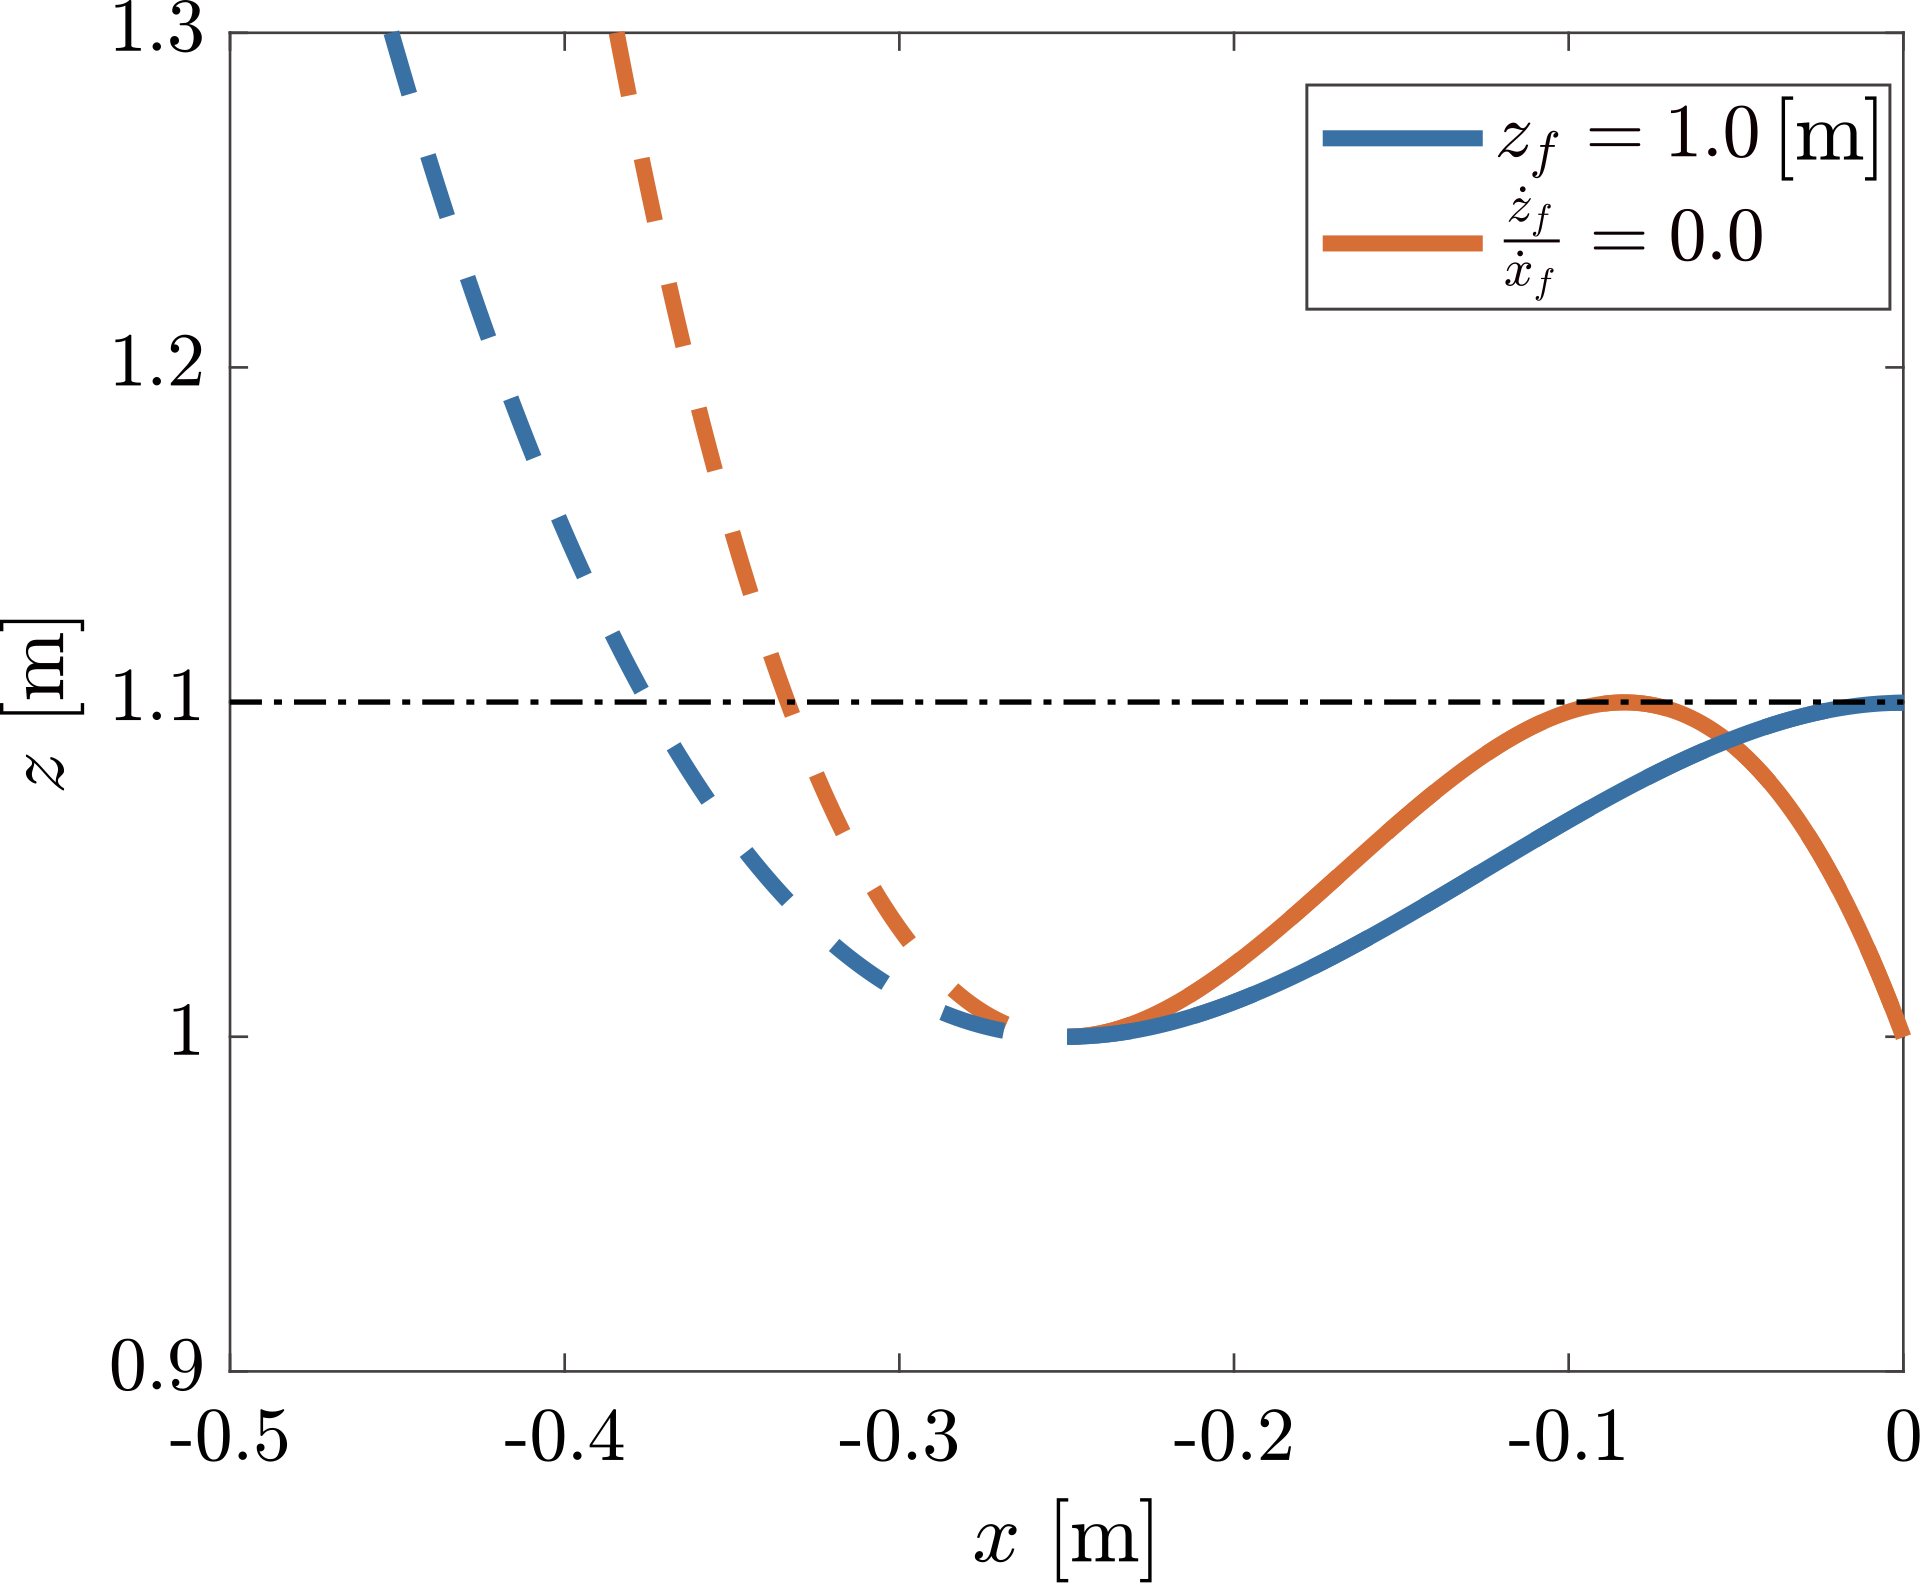
\includegraphics[width=0.6\textwidth]{STYLESTUFF/polynomialHeightViz.png}
\caption{Resulting polynomials as output from Algorithm \ref{alg:h} with two different constraints on the final value. Initial conditions are $x_0=-0.25$ [m], $\dot{x}_0=1.0$ [m/s], $z_0=1.0$ [m] and $\dot{z}_0=0$ [m/s]. Blue plot: $\dot{x}_f=0.552$ [m/s], red plot: $\dot{x}_f=0.576$ [m/s], $z_{max}=1.1$ [m]. }
\label{fig:polheight}
\end{figure}

It is challenging, if not impossible, to find a gradient of the function $\dot{x}_f$. Therefore, the size of increment $\alpha$ cannot be determined based on a gradient. Using the final velocity of the \ac{LIP} orbital energy and a final velocity after the influence of an impact as in $x_{cp,\zmax}$, an increment can be derived. 
The final velocity according to the \ac{LIP} orbital energy is:
\begin{equation}
	\dot{x}_{f,lip} = \sqrt{\dot{x}_0^2-\frac{g}{z}x_0^2},
\end{equation}
where $\dot{x}_{f,lip}$ is the \ac{LIP} final velocity. The final velocity of a height constrained bound as in $x_{cp,\zmax}$ can be calculated as follows:
\begin{equation}
	\dot{x}_{f,\zmax} = \sqrt{\dot{x}_{0,I}^2-\frac{g}{\zmax}(x_0+\frac{\dot{z}_I}{g}\dot{x}_{0,I})^2},
\end{equation}
where $\dot{x}_{0,I}=\dot{x}_0 - \frac{x}{z}\dot{z}_I$ is the initial horizontal velocity influenced by the impact of the lag and $\dot{z}_I = \sqrt{2g\delta \zmax}$ is the vertical impact of the leg that lets the point-mass `just' touch the constraint $\zmax$. The increment $\alpha$ is calculated as a linear set of velocity differences:
\begin{equation}
	\alpha =\frac{\dot{x}_{f,cp} -\dot{x}_{f,\zmax}}{N}
\end{equation}
where the value $N=30$ resulted in reasonable precision, as shown in for example \figref{fig:polheight} and a computation time of an average of $0.51$ [ms] in Java.

% leg length constraint
\subsection{Maximum Leg Length Constraint}
Instead of a constraint on the height of the pendulum, also a constraint on the length can be added as kinematic constraint, which can simulate the maximum leg length. The leg length as a function of $x$ can be expressed using the Pythagorean theorem:
\begin{equation}
	l^2(x) = f(x)^2 + x^2,
\end{equation}
where $l$ the length of the virtual leg. The solution to $f(x)^2$ is:
\begin{equation}
f(x)^2=(\sum_{n=0}^3 c_n x^n)^2 = \sum_{n=0}^3 c_n^2 x^{2n} + 2\sum_{\substack{n=1 \\ i+j=n \\ i < j}}^5 c_i c_j x^n. 
\end{equation}
However, as the gradient of $l^2(x)$ needs to be computed to obtain the locations of the maxima, $f(x)^2$ is approximated with:
\begin{equation*}
	f(x)^2\approx \sum_{n=0}^3 c_n^2 x^{2n}.
\end{equation*}
With this formulation of the squared function, the squared $x$ position in $l(x)^2$ where the maximum pendulum length lies, is computed in the following way:
\begin{align}
	\frac{d(f(x)^2+x^2)}{dx}&=0\\
	\frac{d(f(x)^2+x^2)x}{dx}&=0\\
	6c_3^2 x^4 + 4 c_2^2 x^2 + 2+2c_1^2 &= 0\\
	6c_3^2 (x^2)^2 + 4 c_2^2 (x^2) + 2+2c_1^2 &= 0
\end{align}
Again, the value of the maximum peak lies on the highest $x$ value of the two locations where the gradient is zero, this time in $l(x)^2$. Algorithm \ref{alg:ll} shows how the polynomial constants can be found under the leg length constraint. In Figure \ref{fig:pollength}, it can be seen that the resulting polynomials do not violate the maximum length constraint.
\begin{algorithm}
\caption{Find cubic polynomial constants under leg length constraint}
\label{alg:ll}
\begin{algorithmic}[1]
    \State $\dot{x}_{f}\gets 0$\Comment{Initial guess}
        \Repeat
            \State $\vect{c}\gets \matr{A}^{-1}\vect{b}(\dot{x}_{f})$ \Comment{Find polynomial constants}
            \State $x_{lmax}^2 \gets \frac{-4c_2^2+\sqrt{16c_2^4-24c_3^2(2+2c_1^2)}}{12c_3^2}$ \Comment{$d(f(x)^2+x^2)/dx=0$}  
            \State $x_{lmax}\gets-|\sqrt{x_{l^2max}}|$                \Comment{Complex solutions}
            \State $l_{peak}^2 \gets x_{lmax}^2 + (c_0 + c_1x_{zmax} + c_2x_{zmax}^2+ c_3x_{zmax}^3)^2$ 
            \State $\dot{x}_{f} \gets \dot{x}_{f}+\alpha$   \Comment{Velocity increment}
        \Until{$l_{peak}^2<l_{max}^2$}\\
    \Return $\vect{c}$    
\end{algorithmic}
\end{algorithm}
\begin{figure}[h]
\centering
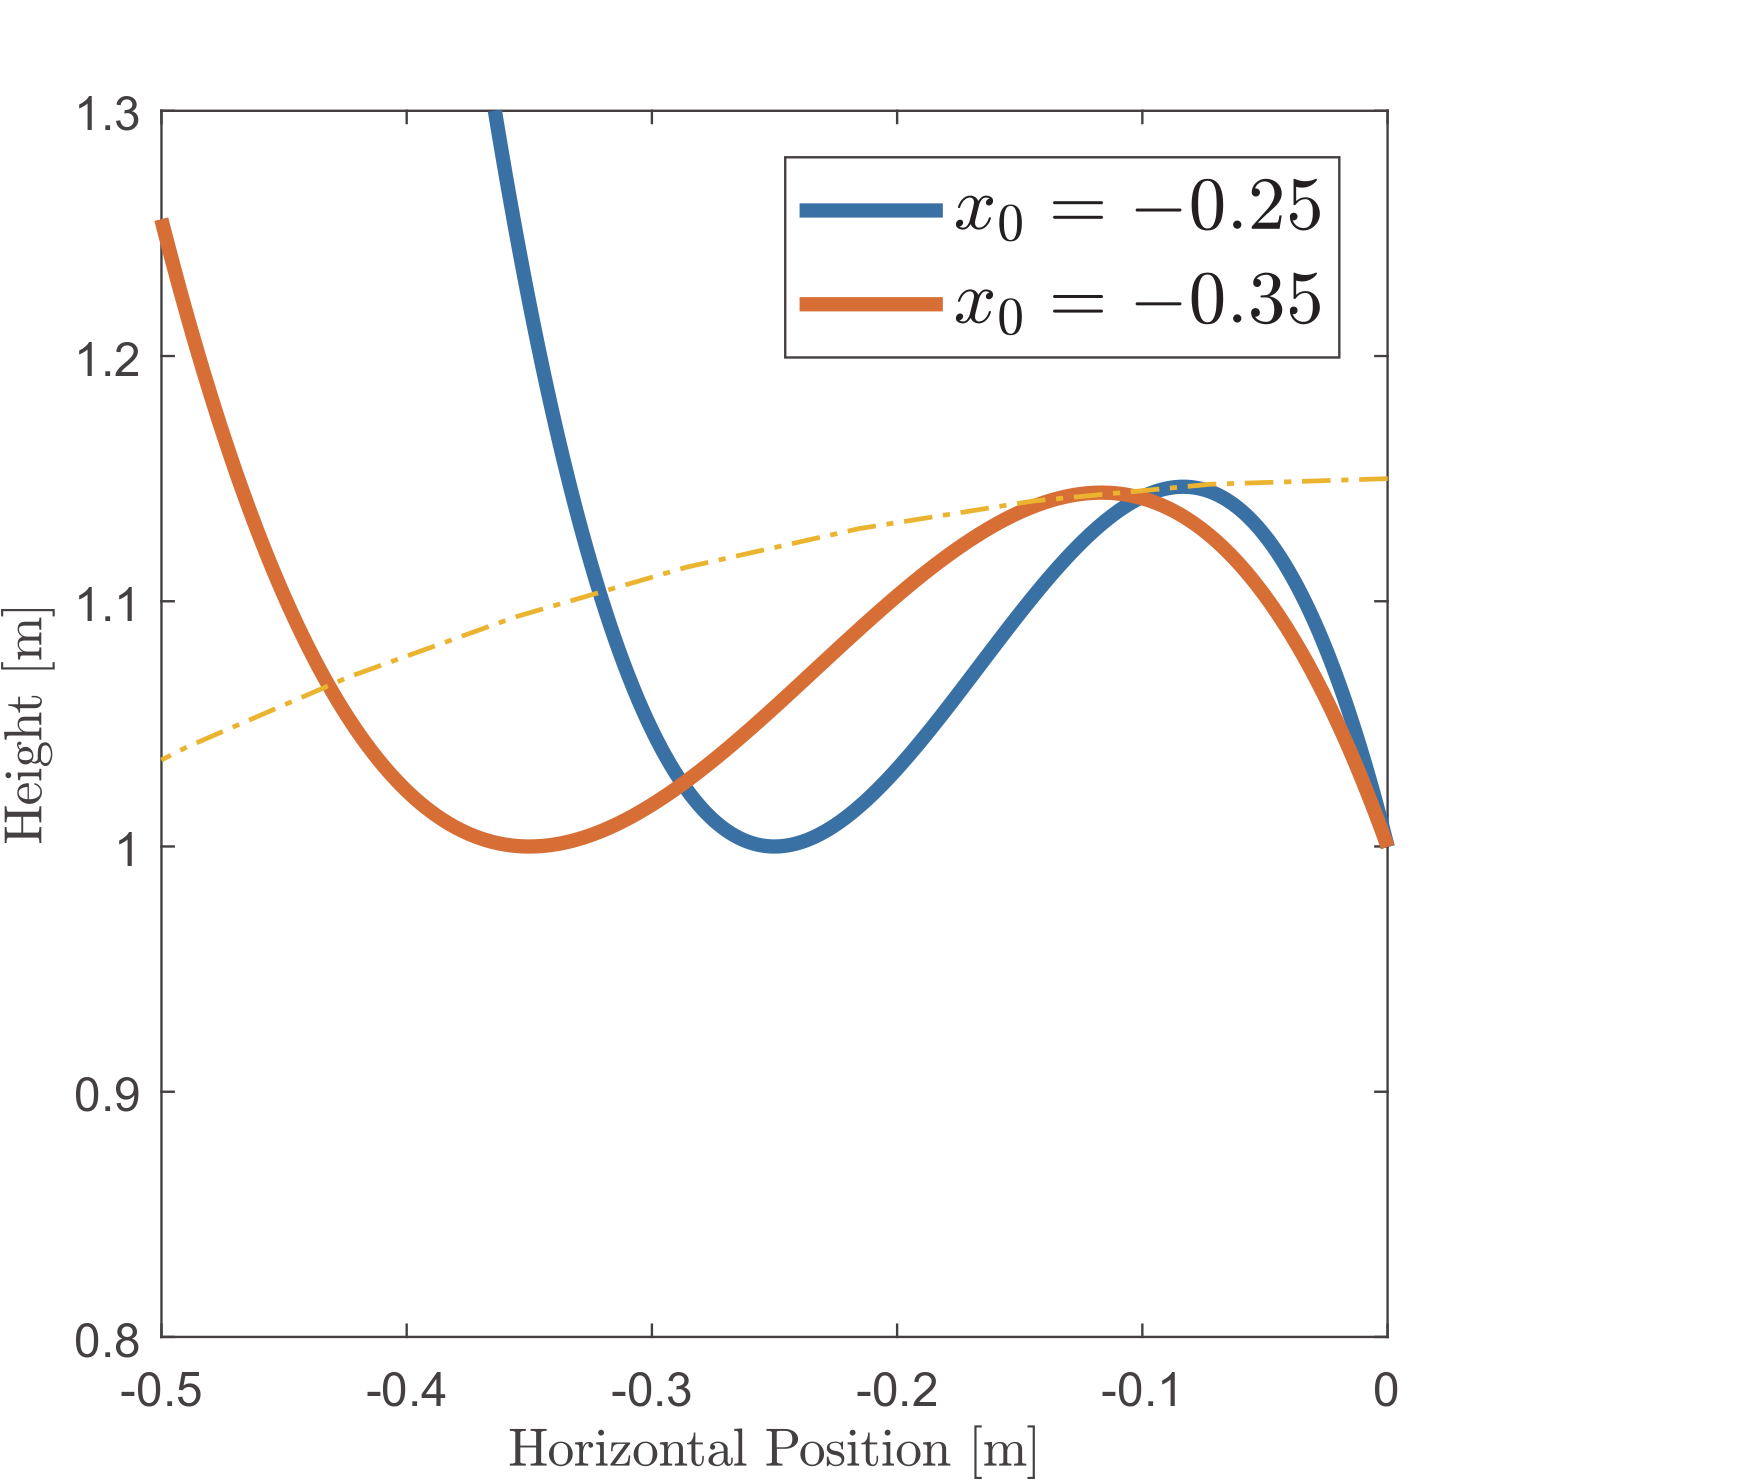
\includegraphics[width=0.6\textwidth]{STYLESTUFF/polynomialLengthViz.png}
\caption{Resulting polynomials as output from Algorithm \ref{alg:ll} with two different initial values under the final height constraint $z_f=1.0$. Other initial conditions are $\dot{x}_0=1.4$ [m/s], $z_0=1.0$ [m] and $\dot{z}_0=0$ [m/s]. Blue plot: $\dot{x}_f=1.107$ [m/s], red plot: $\dot{x}_f=0.724$ [m/s], $l_{max}=1.15$ [m]. }
\label{fig:pollength}
\end{figure}
% discussion
\section{Discussion}
In the chapter, a search algorithm is proposed that is able to find \ac{VHIP} orbital energy trajectories, extending the work in \cite{koolen2016balance}. The horizontal velocity of the orbital energy at $x=0$ is left undetermined, such that this variable could be used in the search. Using the right choice of search increment using knowledge of Chapter \ref{chap:regions}, constrained trajectories could be generated in a time that is suitable for online use. 

Remarkable is that the final gradient constraint gives a higher final velocity $\dot{x}_f$ compared to the default height constraint in \figref{fig:polheight}. This is caused by the polynomial shapes, as the blue plot, under constraint $z_f$, has a steeper gradient in the first part of the trajectory after $x_0$. This is the crucial part in the trajectory for a acceleration or deceleration action in $x$-direction, as is proven in the previous chapter.

Another drawback to the constraint of the polynomial shape is that derivatives of the function, and thus also accelerations, depend on the function itself. In \figref{fig:polforce}, two plots are shown for $\dot{x}_f = 0$ [m/s], together with a plot of the vertical acceleration. The vertical acceleration has a shape that is desirable for a stopping behavior: high acceleration in the beginning of the trajectory and lower later. However, the acceleration at start is unrealistically high, even for an initial position that is relatively close to the \ac{CP}: $x_0=-0.3$ [m]. Also, the vertical acceleration almost does not got below zero, so the polynomial does not make use of higher deceleration, which could lower the amount height variation.
\begin{figure}[h]
\centering
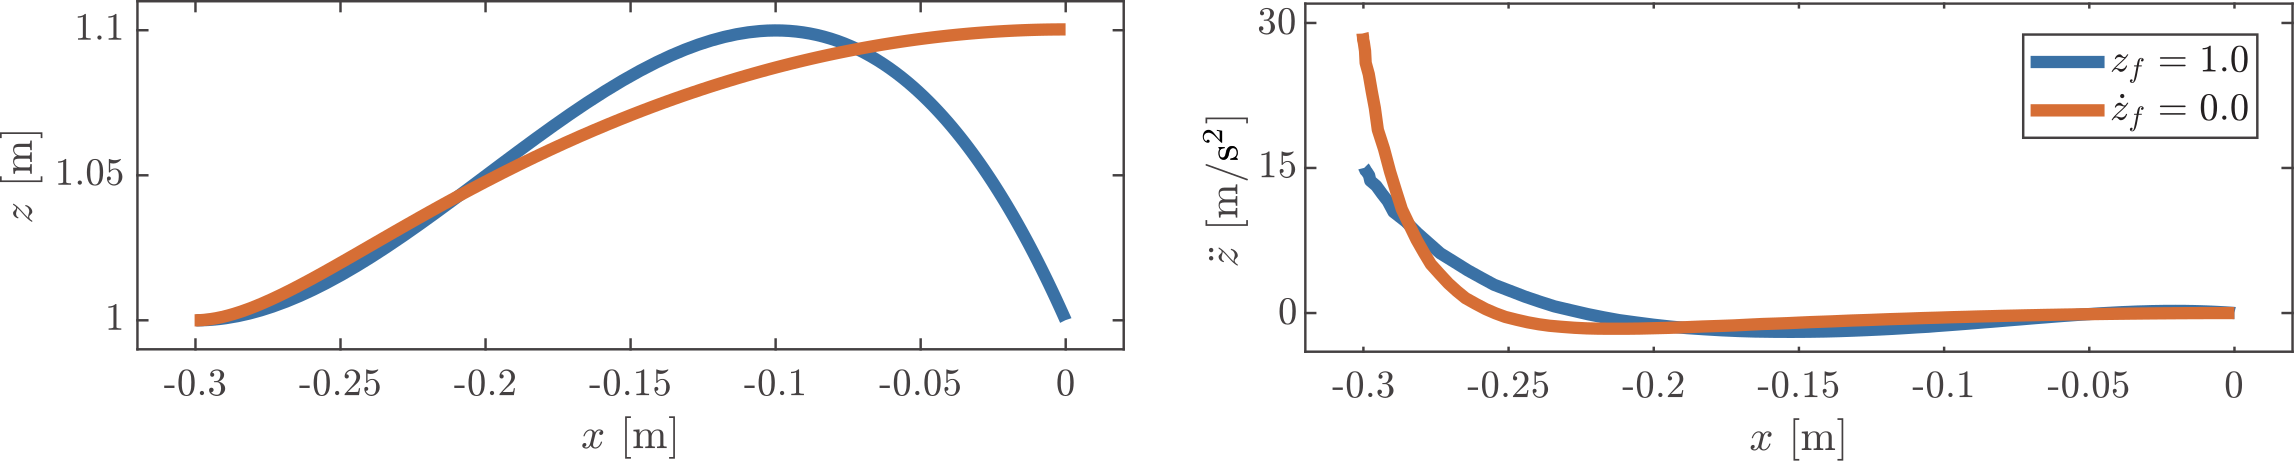
\includegraphics[width=\textwidth]{STYLESTUFF/polynomialforce.png}
\caption{Position plot (left) versus the resulting vertical acceleration (right).}
\label{fig:polforce}
\end{figure}

Also, the orbital energy gives precise knowledge of future states of the \ac{VHIP}. In an applied setting, the desired accelerations on the \ac{CoM} go to multiple control cycles before reaching realized joint torques, like for example the momentum-based whole-body control framework. Having knowledge of the precise differences between the \ac{LIP} and \ac
{VHIP} model over time might be outweighed against all uncertainties that come with the real system. 

For those reasons, the methods proposed in this chapter are not used in application in Chapter \ref{chap:standing} and Chapter \ref{chap:walking}.
